% !Mode:: "TeX:UTF-8"

\chapter{基于BlazePose的人体姿态估计算法研究}

\section{推理通道}

在推断过程中,采用了detector-tracker设计。流程(见图~\ref{piture:11}~)包括一个轻量级的人体姿态估计检测器,和一个紧随其后的姿态跟踪网络。当目前帧上有人体出现时,使用跟踪网络预测关键点坐标;当跟踪器不能检测出关键点坐标,即没有人出现时,检测器会在下一帧重新启用。

具体来说,模型会使用检测器定位图像的姿态ROI,然后传给跟踪器,预测出33个关键点的坐标。对于视频流来说,检测器只会在第一次出现人脸之前运行。对于检测到人脸之后,会从前一帧的33个关键点中预测出ROI。

\begin{figure}
\centering
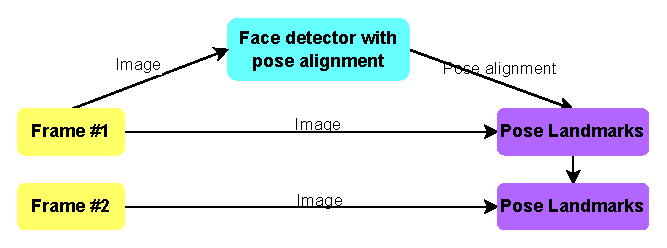
\includegraphics[width=1\linewidth]{Inference_pipeline}
\caption{推理通道}
\label{piture:11}
\end{figure}

\section{神经网络结构}

我们将两种主流的方法,即基于热图和基于回归相结合,如图~\ref{piture:12}~所示。热力图所在的网络层只在训练过程中出现,不包含回归。当训练完成时,热力图相对应的输出层将会被删除,从而降低模型的复杂度,提升模型的轻量化。同时,还使用了堆叠沙漏方法\cite{newell2016stacked},但与之不同的是,本项目同时堆叠了一个encoder-decoder热图网络和一个回归encoder网络。

\begin{figure}
\centering
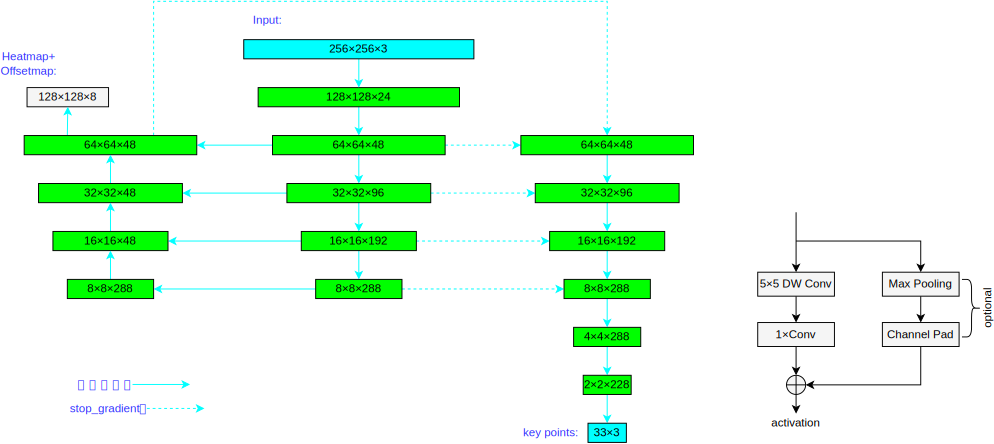
\includegraphics[width=1\linewidth]{model}
\caption{神经网络结构}
\label{piture:12}
\end{figure}

中间上面是输入图片,然后逐步向下,是个bottom-up的过程,每个scale都有向左和向右的横向链接。

左边从下到上,是个top-down的过程,和中间部分有横向链接skip connections,这都和``Hourglass''一样,最上面是``Hourglass''部分输出的heatmap,这个heatmap仅仅用来应用loss监督训练``Hourglass''部分生成中间的embedding特征,在预测以及regression部分都不参与。

右边从上到下整个是regression encoder网络,这部分不参与训练``Hourglass''部分,仅仅用来``后处理''。它每层有对应的输入,其中最上面的第一层输入来自两部分,分别是bottom-up以及top-down的同级分辨率特征(heatmap没有参与过来,也就是砍掉了),最后输出33个关键点信息。

从图~\ref{piture:12}~中可以看出,本项目的模型,充分连接了网络的各个阶段,使其不再孤立,从而平衡了深浅层的特征。不同层次之间存在跨层连接,这样既可以发挥深层网络的特化语义信息,抽象信息;也可以充分发挥浅层网络提取出的细粒度的边缘、颜色、转角、斑块,这些底层的图像信息。图中的实线是残差连接,即可以回传梯度,虚线表示停止回传梯度。这样使得热图的预测准确率和坐标的精度都大大提升。

图~\ref{piture:13}~和图~\ref{piture:14}~分别展示了本项目模型每层的连接关系和每一层的具体实现细节。可以看出网络一共由二十三层,其中Conv7a至Conv11为热力图分支,Conv11为热力图输出,Conv12a至Conv15为回归分支,Conv15为全连接层。中间层激活函数均为Relu,最后一层的激活函数为Sigmoid。

\begin{figure}
\centering
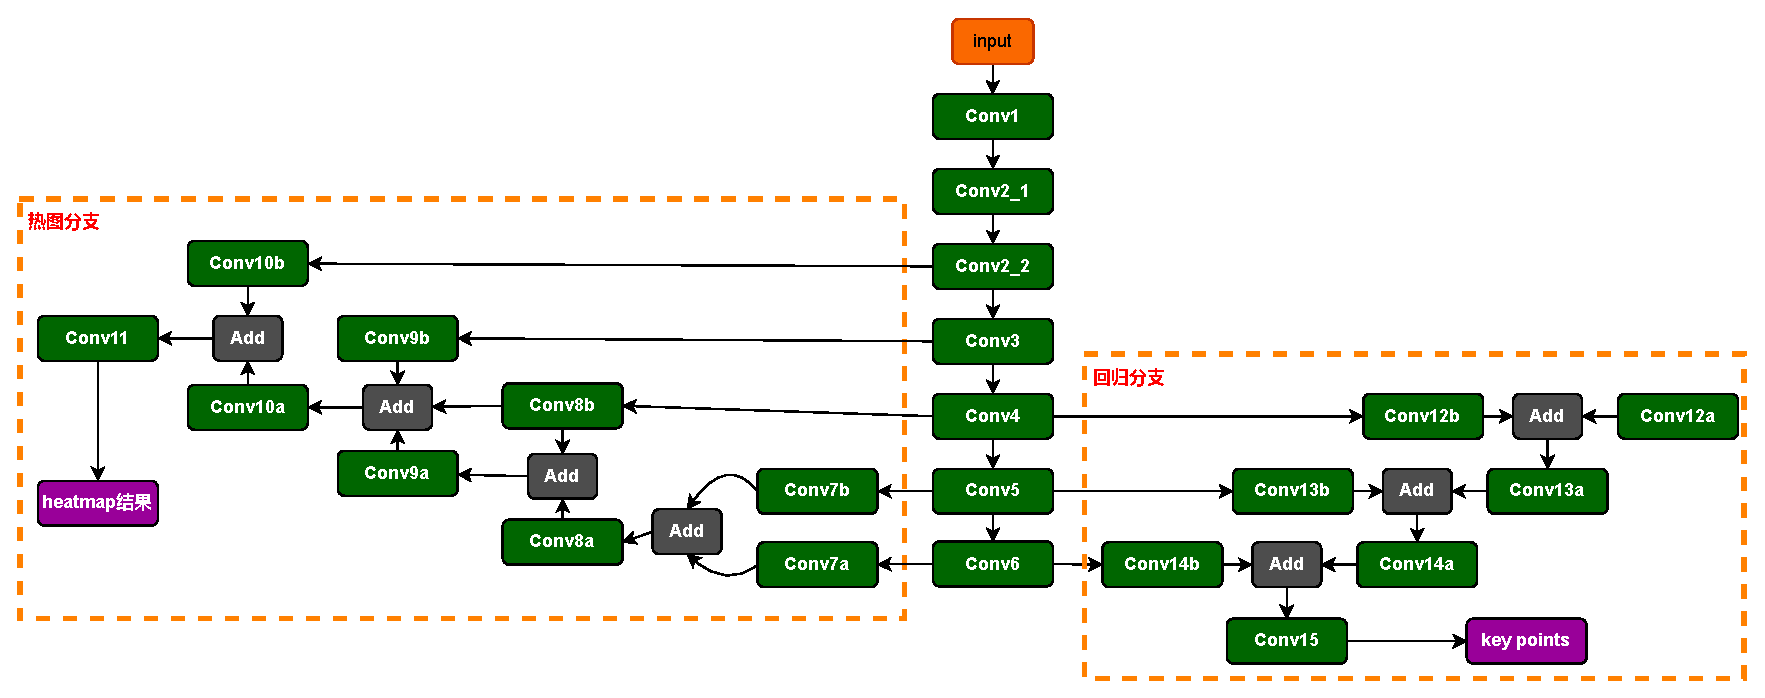
\includegraphics[width=1.1\linewidth]{network-architecture-simple}
\caption{层与层之间的连接关系}
\label{piture:13}
\end{figure}

\begin{figure}[!h]
	\centering
	\begin{sideways}
		\begin{minipage}{\textheight}
			\centering
			\fbox{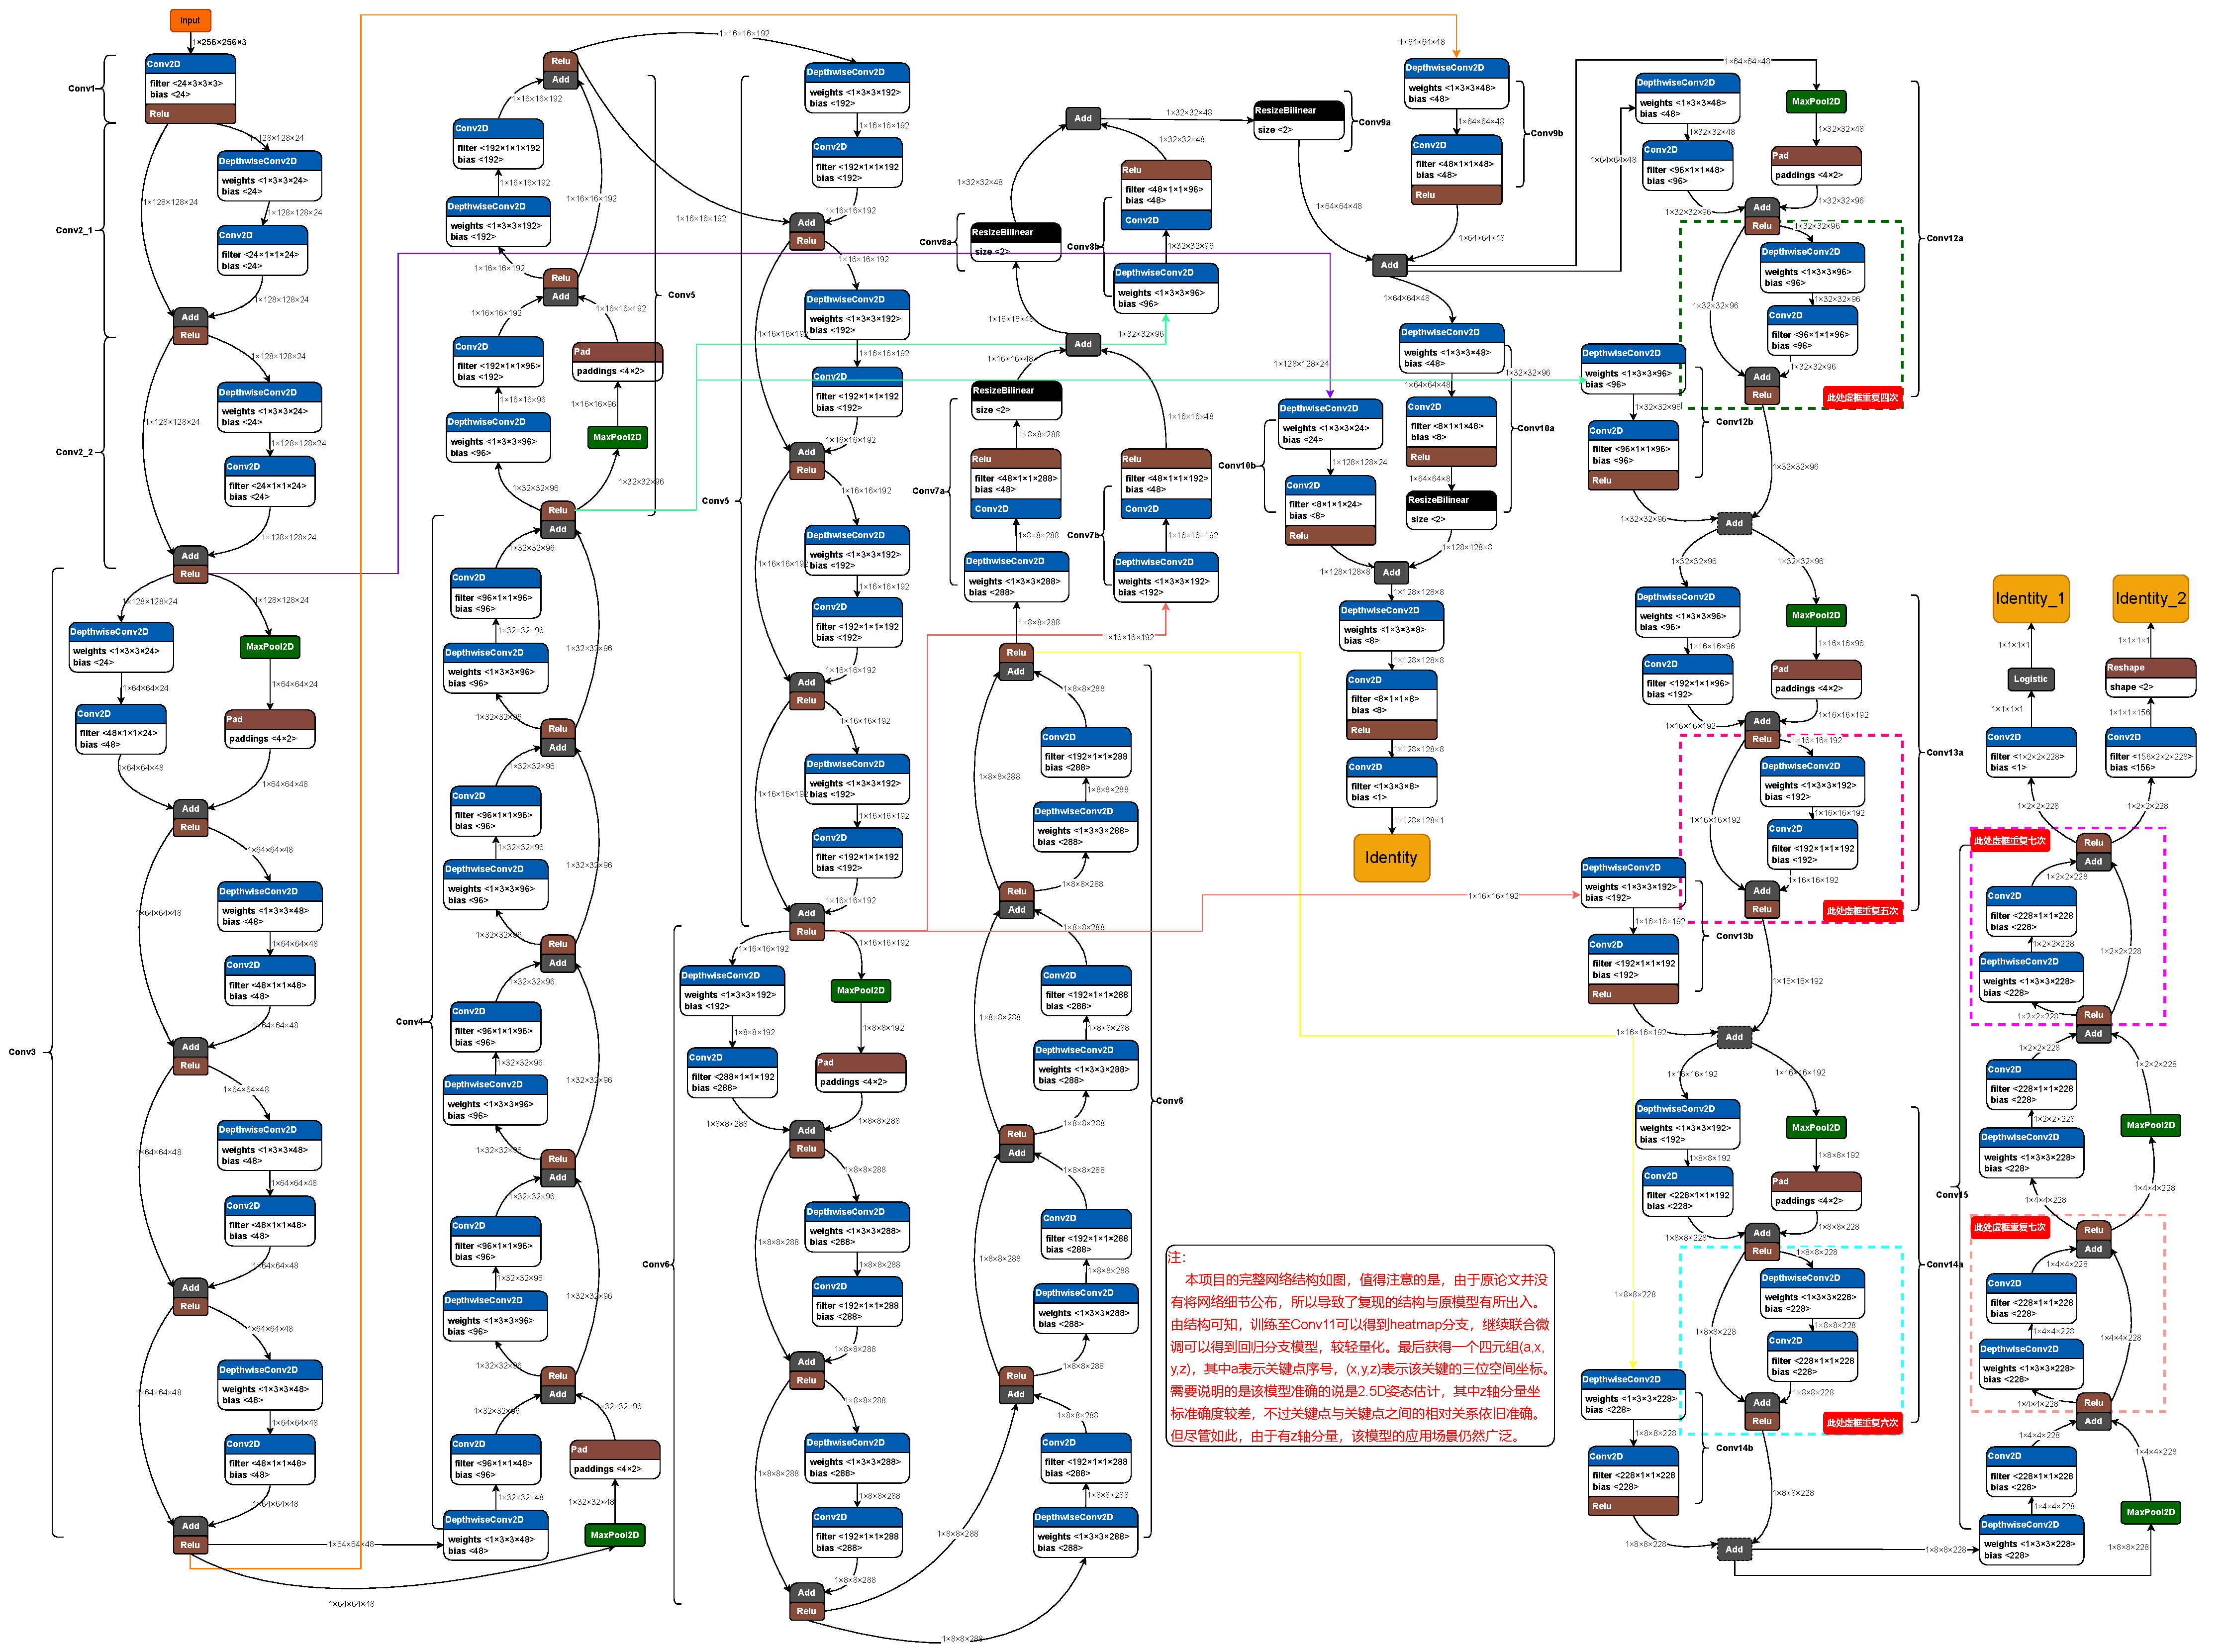
\includegraphics[width=0.9\textwidth]{network-architecture-full}}
			\caption{层与层之间的连接关系和每层的实现细节}
			\label{piture:14}
		\end{minipage}
	\end{sideways}
\end{figure}

\section{人体检测器}

目前主流的人体姿态估计算法在检测人体的后处理步骤中,都是使用的NMS算法,不过NMS对于非刚性物体并不是很友好,尤其是类似与人体这类关节复杂度高的姿势场景。这是因为有大量的,模糊的候选框都满足非最大值抑制的交并比阈值。

因此,本项目摒弃了NMS算法,而采用人脸检测框。这是因为在大多数情况下,人脸较为刚性,是关于躯干的最强信号。因此,我们做出了一个假设,即在单人姿态估计中,人脸是必须要出现的。

该检测器(见图~\ref{piture:15}~)来自谷歌的轻量级BlazeFace模型,它预测了人体两个髋关节的中点作为整个人体的中心,并以此为圆心,画一个能够包含整个人体的最小圆,这就是本项目中的ROI。对于人体倾斜的情况,还预测了人体中心与两个眼睛的中心之连线和铅垂线的夹角,将图像旋转这个夹角即可得到标准的人体图像。

\begin{figure}[htbp]
\centering
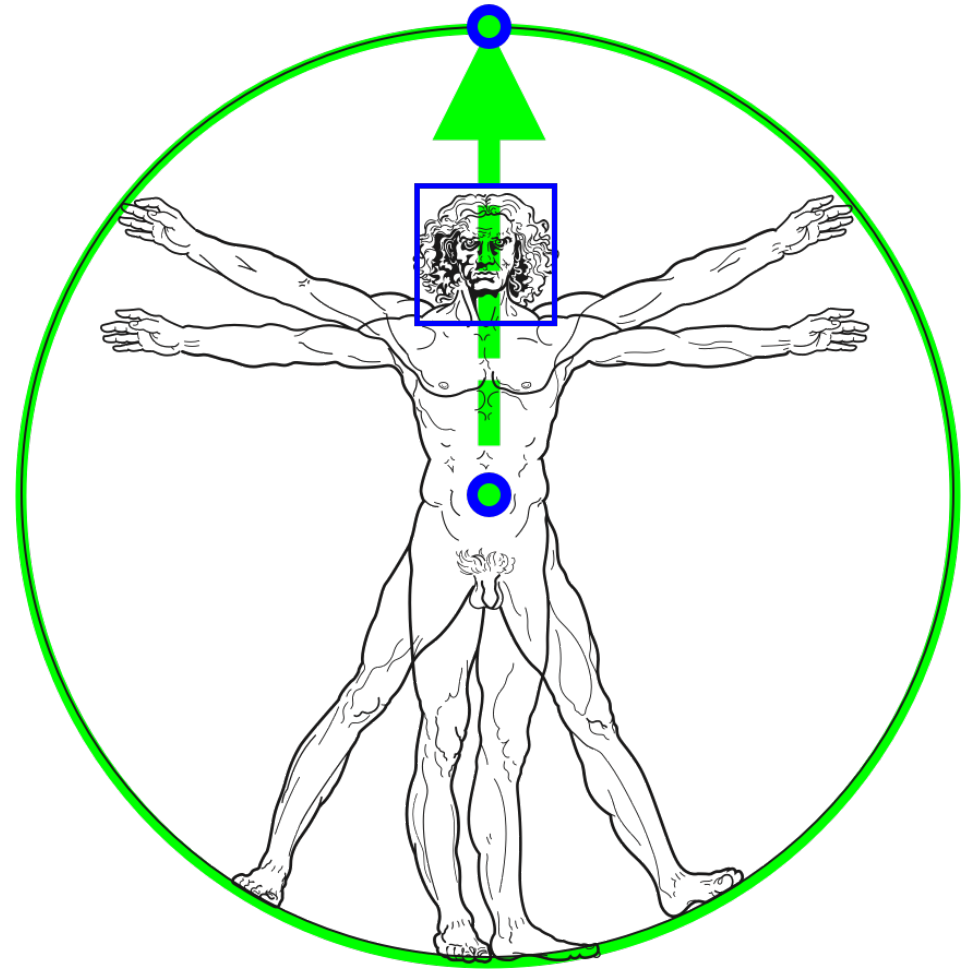
\includegraphics[width=0.6\linewidth]{human}
\caption{从维特鲁威人中受到启发的检测器}
\label{piture:15}
\end{figure}

\section{人体拓扑结构}
我们结合了BlazeFace、BlazePalma和Coco使用的数据集,并研究了他们的并集之超集,提出了人体33个关键点。

和OpenPose\cite{8765346}以及Kinect\cite{zhang2012microsoft}的关键点不同的是,本文在脸部,手部和脚部添加了更多的关键点,用来估计后续模型的ROI。拓扑结构如图 \ref{piture:16}所示。

\begin{figure}
\centering
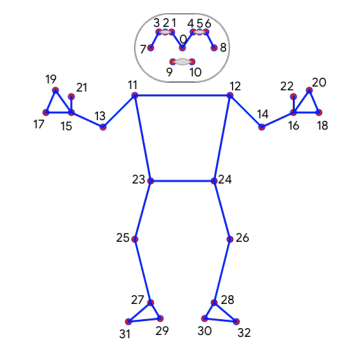
\includegraphics[width=0.6\linewidth]{keypoints}
\caption{33个关键点}
\label{piture:16}
\end{figure}

此外,各个关键点的名称详见附录1\fcolorbox{red}{white}{~\nameref{keypoints}~}。

\section{输入输出}
由复现的网络结构图~\ref{piture:14}~可知,模型的输入是:

视频帧中检测到人的区域。大小是$256\times256\times3$,在垂直身体姿势中以两个髋关节的中部为中心。 通道顺序是RGB。

模型的输出是33对3元组$(X,Y,Z)$,其中33对表示33个关键点,3对分别是关键点在$X,Y,Z$轴上的坐标:

\begin{enumerate}
\item $X,Y$坐标是感兴趣区域的局部坐标,范围为$[0.0,255.0]$;

\item $Z$坐标与$X$和$Y$坐标一样以``图像像素''测量,表示相对于臀部平面的距离。正值表示在臀部的后面,负值表示在臀部和相机之间。这样就可以知晓33个关键点,尤其是手部和腿部的$Z$轴位置,可以充分发挥图像的信息。但$Z$坐标与$X$和$Y$坐标不一样的是,$X$和$Y$坐标通过人工注释获得,而$Z$坐标是通过将合成数据(GHUM模型\cite{xu2020ghum,zanfir2020weakly})拟合到2D模型中,是按比例计算的。
\end{enumerate}

\section{本章小结}
在本章中,我们对BlazePose算法做出了细致的研究,包括其推理通道,神经网络结构,人检测器,关键点模型等等,其中着重介绍了本项目复现出的神经网络结构。

% Local Variables:
% TeX-master: "../main"
% TeX-engine: xetex
% End:
